\documentclass[letterpaper,10pt]{article}

\usepackage{enumitem}
\usepackage{titling}
\usepackage{listings,listings-rust}
\usepackage{url}
\usepackage{soul}
\usepackage{hyperref}
\usepackage{setspace}
\usepackage{subfig}
\usepackage{sectsty}
\usepackage{pdfpages}
\usepackage{colortbl}
\usepackage{multirow}
\usepackage{multicol}
\usepackage{relsize}
\usepackage{amsmath}
\usepackage{wasysym}
\usepackage{fancyvrb}
\usepackage[yyyymmdd]{datetime}
\usepackage{amsmath,amssymb,amsthm,graphicx,xspace}
\usepackage[titlenotnumbered,noend,noline]{algorithm2e}
\usepackage[compact]{titlesec}
\usepackage{XCharter}
\usepackage[T1]{fontenc}
\usepackage[scaled]{beramono}
\usepackage[normalem]{ulem}
\usepackage{booktabs}
\usepackage{tikz}
\usetikzlibrary{arrows.meta,automata,shapes,trees,matrix,chains,scopes,positioning,calc,decorations.pathreplacing}
\tikzstyle{block} = [rectangle, draw, fill=blue!20, 
    text width=2.5em, text centered, rounded corners, minimum height=2em]
\tikzstyle{bw} = [rectangle, draw, fill=blue!20, 
    text width=4em, text centered, rounded corners, minimum height=2em]

\definecolor{namerow}{cmyk}{.40,.40,.40,.40}
\definecolor{namecol}{cmyk}{.40,.40,.40,.40}
\renewcommand{\dateseparator}{-}

\let\LaTeXtitle\title
\renewcommand{\title}[1]{\LaTeXtitle{\textsf{#1}}}

\lstset{basicstyle=\footnotesize\ttfamily,breaklines=true}

\newcommand{\CPP}{C\nolinebreak\hspace{-.05em}\raisebox{.4ex}{\tiny\bf +}\nolinebreak\hspace{-.10em}\raisebox{.4ex}{\tiny\bf +}}
\def\CPP{{C\nolinebreak[4]\hspace{-.05em}\raisebox{.4ex}{\tiny\bf ++}}}

\newcommand{\handout}[5]{
  \noindent
  \begin{center}
  \framebox{
    \vbox{
      \hbox to 5.78in { {\bf ECE459: Programming for Performance } \hfill #2 }
      \vspace{4mm}
      \hbox to 5.78in { {\Large \hfill #4  \hfill} }
      \vspace{2mm}
      \hbox to 5.78in { {\em #3 \hfill \today} }
    }
  }
  \end{center}
  \vspace*{4mm}
}

\newcommand{\lecture}[3]{\handout{#1}{#2}{#3}{Lecture #1}}
\newcommand{\tuple}[1]{\ensuremath{\left\langle #1 \right\rangle}\xspace}

\addtolength{\oddsidemargin}{-1.000in}
\addtolength{\evensidemargin}{-0.500in}
\addtolength{\textwidth}{2.0in}
\addtolength{\topmargin}{-1.000in}
\addtolength{\textheight}{1.75in}
\addtolength{\parskip}{\baselineskip}
\setlength{\parindent}{0in}
\renewcommand{\baselinestretch}{1.5}
\newcommand{\term}{Winter 2023}

\singlespace


\begin{document}

\lecture{9 --- Algorithms, Concurrency, and Parallelism}{\term}{Jeff Zarnett, based on original by Patrick Lam}

\section*{Algorithms}
Remember from ECE~250/CS~138 that we often care about the worst case run-time performance of the algorithm. A bad algorithm has terrible runtime characteristics for a large data set. Trying to do an insertion sort on a small array is fine (actually... recommended); doing it on a huge array is madness. Choosing a good algorithm is very important if we want it to scale.  But you know that already; you're not in a 4\textsuperscript{th} year engineering course to have me tell you that you can use quicksort rather than bubble sort.

\begin{center}
	\includegraphics[width=0.75\textwidth]{images/big-o-complexity}\\
	Big-O Complexity comparison from ~\cite{bigocheatsheet}
\end{center}

Sorting is probably a bad example, though, because in a non-university-course situation, you almost certainly use a library- or language-provided implementation and you can just call \texttt{sort()} on the collection and it's done for you. But what about other situations?

While I [JZ] am not generally a fan of leetcode-style interviews as a way of determining aptitude for a job, there are some good ideas in how to approach that sort of interview that \textit{can} be applied in real life. The objection I have is not that this is something you \textit{never} do -- just that it happens somewhat rarely and much more time will be spent on architecture or just figuring out what the needs of the user are. But anyway! Here's the basics of what I advise people when preparing for such an interview, and it applies well to non-interview situations.

The best place to start is likely a simple solution, which may be brute-force. In many scenarios, that's adequate because the code in question is not performance-critical or the order of magnitude of $n$ in the Big-O notation is sufficiently small that it doesn't matter. Given a working (correct) implementation, if you then discover it's not working performance-wise, the next step is to refine it. 

Refinement here means to improve the algorithm you've got. The book \textit{Cracking the Coding Interview}~\cite{mcdowell2015cracking} uses the acronym BUD for this: Bottlenecks, Unnecessary Work, Duplicated Work. Let's look at those things a bit.

A bottleneck is exactly what it sounds like, a rate-limiting part of the code. If we could improve that, we'd get the most benefit. If your code has multiple phases (do $X$, then do $Y$, then do $Z$), figuring out which of these is the slowest one helps. If $X$ is load data, $Y$ is to do some transformation of it, and $Z$ is send the data over the network -- optimizing sending doesn't accomplish much if the slowest part is loading data. 

Unnecessary work is also straightforward to define: any work that we did that isn't necessary. If we found the data element we need in the array we can stop looking now: anything else is wasted effort. That sort of thing doesn't change the algorithmic complexity, but it does reduce the total time of execution. Or another example would be considering data where we can tell in advance it's not going to work out -- like a real-time system that won't schedule a task that has no hope of meeting its deadline.

And finally, duplicated work is anything more than once. Re-computing a value when you could remember that result instead is an easy example -- even if the compiler might bail you out there. A more realistic example is if you repeatedly search an array, maybe putting all the data in a hashmap first saves a lot of effort. 

In a coding-interview situation, you have a well-defined set of pieces of information. Chances are, you need to use all of them to find optimal solution. In other situations, it's not provided for you in the same way, so you may need to investigate. As an example, a coding problem might say that the array is sorted on the \texttt{id} field in ascending order. That might be true of the data you're getting in the function you're writing, but you may have to do some research or investigation to find out if that's the case, or maybe you need to be the change you want to see and add a call to sort the data.

Most of the discussion of Big-O complexity assumes a large enough $n$ in the situation that the other terms don't matter. That's fine for an interview, but is not always true in real life. Sorting a large array or putting it into a Hashmap is likely to be optimal if you intend to use it many times, but maybe is not worthwhile if we just need to search it once. 

It is also possible, as (sometimes) in a coding interview, to ask for help, if stuck. Another look or the eyes of a more senior colleague can help you spot an improvement or idea (or just help you get there faster). 

Remember also that algorithmic complexity improvements always have limits. For ECE~459 at the end of the term, to successfully mark the final exam, the teaching team really does have to look at every question of every exam paper. No amount of cleverness in the process -- switching to Crowdmark rather than marking on paper, for example -- can get around the fact that the only way to properly mark the exam is to look at every single question as answered by each student. So this has linear runtime and we can never do any better than that. 

\subsection*{System Design}
Sometimes when you look at the situation, you'll find the reason that the runtime is what it is has to do with the design of the larger system in which the data lives. For example, if we have to do a lot of network calls to get the data that's needed that will increase the time to do the operation compared to getting all the data locally or in only one network call. 

Whether you can change the data layout or the system architecture is very situation-dependent. It is generally unlikely that you will be able to convince your company to split up their five year old monolith codebase because it would be faster in some scenarios -- the opportunity cost is large. Similarly, it might be optimal for your use case to change how the data is represented in the database, but worse for another, more common, use case and so the structures won't change. 

System design interviews are another popular screening method for candidates in industry. I [JZ] like this better than the leetcode interviews in terms of understanding a candidate's ability to do the (typical) work of software development. While choosing a good or bad architecture will obviously affect the performance of the system, that topic is better left to an architecture course.

\subsection*{Accidentally Quadratic}
Given that many problems really are linear at the core (take an item, do something with it, go on to the next), a problem arises when we combine two linear things and get quadratic behaviour. Oh no! This is a situation that can be described as ``accidentally quadratic''.

There are a number of good examples at \url{https://accidentallyquadratic.tumblr.com/} if you are interested in seeing some more, though they are in different languages and the most recent post seems to be from mid-2019. To find a Rust-specific example, I had to go pretty far back in the archives and came up with this one from 2016(!): \url{https://accidentallyquadratic.tumblr.com/post/153545455987/rust-hash-iteration-reinsertion}. Let's recap their explanation:

Rust's hash tables used a strategy called \textit{Robin-Hood Hashing}\footnote{See this paper! \url{https://cs.uwaterloo.ca/research/tr/1986/CS-86-14.pdf}}, which is based on open addressing with linear probing. Remember that open addressing is finding an alternate location in the event of a collision, rather than chaining and linear probing means you start from the bucket we should land in and move forward until you find a free space. The Robin-Hood part says if we have an item that's farther from its intended bucket than the current item, swap them. So if the order of items is 2 - 0 - 1, we'll swap until 0 - 1 - 2. This reduces the variance of items -- how far away from where they ``should'' be on average.

Suppose you want to copy the data to a new hash table. To illustrate the problem, start by copying the data to a table half the size of the original. This works fine for the first half, but then as the second hash table is getting full we have to scan longer and longer to find the right place for it to go. Because this linear scan of finding a free bucket is already within the linear loop of ``copy all items from table one to table two'' we have indeed found an accidentally quadratic situation. When the second table is full enough to trigger a resize, then the problem goes away... at least until the table is almost full. See the time taken diagram:

\begin{center}
  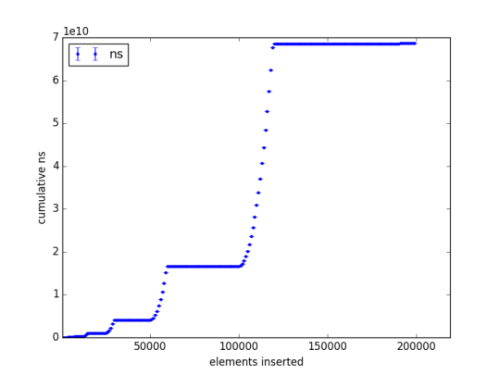
\includegraphics[width=0.5\textwidth]{images/robinhoodhashing.png}
\end{center}

That certainly looks quadratic. Not all the time, of course, but that doesn't matter. Algorithmic analysis is all about the worst-case scenario and sometimes when we insert things into this table it's quadratic and that's bad. 

Not convincing? A simpler version of this looks something like: given a large number of elements to insert to an almost-full hash table, the runtime becomes quadratic because for each element you have to do a linear search to find where to insert it.

Now... please don't over-index on this one example to the point that you're arguing with your interviewer that \textit{Well, actually} a hashmap doesn't help and that your solution without one is better. It's just that the real world has nuance and unexpected interactions that mean sometimes the normally-best approach is not the best this time. 

If we can't do any better than linear (or maybe even quadratic), what do we do? Going back to the exam marking example: if I [JZ] had to mark 400+ exams myself, sequentially, I don't know how I'd do it... Or at least it would take so long that I'd get a nasty letter from the Registrar's Office about grades being due. I've got help, though, from the rest of the teaching team (co-instructors, TAs, LI). We divide up the work to finish on time. So -- parallelism!


\section*{Concurrency and Parallelism}
Concurrency and parallelism both give up the
total ordering between instructions in a sequential program, for
different purposes. We're going to focus on threads, but if you need a review of the details and differences of processes vs threads, you might like to read   \url{https://www.purplealienplanet.com/node/50}. 

\paragraph{Concurrency.} We'll refer to the use of threads for
structuring programs as concurrency. Here, we're not aiming
for increased performance. Instead, we're trying to write the program
in a natural way. Concurrency makes sense as a model for distributed
systems, or systems where multiple components interact, with no ordering
between these components, like graphical user interfaces.

\paragraph{Parallelism.} We're studying parallelism in this class, where
we try to do multiple things at the same time in an attempt to increase
throughput. Concurrent programs may be easier to parallelize.

\subsection*{Limits to parallelization}
I mentioned briefly in Lecture 1 that programs often have a sequential
part and a parallel part. We'll quantify this observation today
and discuss its consequences.


\paragraph{Amdahl's Law.} One classic model of parallel execution
is Amdahl's Law. In 1967, Gene Amdahl argued that improvements in
processor design for single processors would be more effective than
designing multi-processor systems. Here's the argument. Let's say that
you are trying to run a task which has a serial part, taking fraction 
$S$, and a parallelizable part, taking fraction $P = 1-S$. Define $T_s$
to be the total 
amount of time needed on a single-processor system.
Now, moving to a parallel system with $N$ processors, the parallel
time $T_p$ is instead:
\[ T_p = T_s \cdot (S + \frac{P}{N}). \]
{\bf As $N$ increases, $T_p$ is dominated by $S$, limiting potential
speedup.}

We can restate this law in terms of speedup, which is the 
original time $T_s$ divided by the sped-up time $T_p$:
\[ \mbox{speedup} = \frac{T_s}{T_p} = \frac{1}{S+P/N}. \]
Replacing $S$ with $(1-P)$, we get:
\[ \mbox{speedup} = \frac{1}{(1-P)+P/N}, \]
and
\[ \mbox{max speedup} = \frac{1}{(1-P)}, \]
since $\frac{P}{N} \rightarrow 0$.

\paragraph{Plugging in numbers.} If $P = 1$, then we can indeed get good
scaling; running on an $N$-processor machine will give you a speedup
of $N$. Unfortunately, usually $P < 1$.  Let's see what happens.

\begin{center}
\begin{tabular}{r|r}
$P$ & speedup ($N=18$) \\ \hline
1 & 18 \\
0.99 & $\sim$ 15 \\
0.95 & $\sim$ 10 \\
0.5 & $\sim$ 2
\end{tabular}
\end{center}
Graphically, we have something like this:
\begin{center}
  \includegraphics[width=0.5\textwidth]{images/parallel-scaling}
\end{center}


Amdahl's Law tells you how many cores you can hope to leverage in an
execution given a fixed problem size, if you can estimate $P$.

Let us consider an example from~\cite{mte241}: Suppose we have a task that can be executed in 5~s and this task contains a loop that can be parallelized. Let us also say initialization and recombination code in this routine requires 400~ms. So with one processor executing, it would take about 4.6~s to execute the loop. If we split it up and execute on two processors it will take about 2.3~s to execute the loop. Add to that the setup and cleanup time of 0.4~s and we get a total time of 2.7~s. Completing the task in 2.7~s rather than 5~s represents a speedup of about~46\%. Applying the formula, we get the following run times:

\begin{center}
	\begin{tabular}{r|l}
	\textbf{Processors} & \textbf{Run Time (s)} \\ \hline
	1 & 5\\
	2 & 2.7\\
	4 & 1.55\\
	8 & 0.975\\
	16 & 0.6875 \\
	32 & 0.54375 \\
	64 & 0.471875 \\
	128 & 0.4359375\\
	\end{tabular}
\end{center}

   \paragraph{Empirically estimating parallel speedup $P$.}
Assuming that you know things that are actually really hard to know, here's a formula for estimating speedup. You don't have to commit it to memory:
  \[P_{\mbox{\scriptsize estimated}} = \frac{\frac{1}{\mbox{\em speedup}}-1}{\frac{1}{N}-1}.\]

It's just an estimation, but you can use it to guess the fraction of parallel code, given $N$ and the speedup. You can then use $P_{\mbox{\scriptsize estimated}}$ to predict speedup for a different number of processors.

\paragraph{Consequences of Amdahl's Law.}
For over 30 years, most performance gains did indeed come from
increasing single-processor performance. The main reason that we're
here today is that, as we saw a few classes ago,
single-processor performance gains have hit the wall.

By the way, note that we didn't talk about the cost of synchronization
between threads here. That can drag the performance down even more.

\paragraph{Amdahl's Assumptions.}
Despite Amdahl's pessimism, we still all have multicore computers today.
Why is that? Amdahl's Law assumes that:
\begin{itemize}[noitemsep]
    \item problem size is fixed (read on);
    \item the program, or the underlying implementation, behaves the same on 1 processor as on $N$ processors; and
    \item that we can accurately measure runtimes---i.e. that overheads don't matter.
\end{itemize}

% replace Amdahl's law with how branch predictors work
\paragraph{Generalizing Amdahl's Law.} We made a simplification,
which was that programs only have one parallel part and one serial part.
Of course, this is not true. The program may have many parts,
 each of which we can tune to a different degree.

Let's generalize Amdahl's Law:

\begin{itemize}
\item  $f_1, f_2, \ldots, f_n$: fraction of time in part $n$
\item  $S_{f_1}, S_{f_n}, \ldots, S_{f_n}$: speedup for part $n$
\end{itemize}

Then,
\[\mbox{\em speedup} = \frac{1}{\frac{f_1}{S_{f_1}} + \frac{f_2}{S_{f_2}} + \ldots +
     \frac{f_n}{S_{f_n}}}.\]

\paragraph{Example.} Consider a program with 4 parts in the following scenario:

\begin{center}
     \begin{tabular}{r|r|r|r}
     \multicolumn{2}{l}{} & \multicolumn{2}{|c}{Speedup} \\
     Part & Fraction of Runtime & Option 1 & Option 2\\
     \hline
     1 & 0.55 & 1  & 2\\
     2 & 0.25 & 5  & 1\\
     3 & 0.15 & 3  & 1\\
     4 & 0.05  & 10 & 1\\
     \end{tabular}
 \end{center}

     (Note: these speedups don't have to be speedups from parallelization.)
    
   We can implement either Option 1 or Option 2. 
   Which option is better?

   ``Plug and chug'' the numbers:
 \begin{itemize}
 \item  {\bf Option 1.}

   \[ \mbox{\em speedup} = \frac{1}{0.55 + \frac{0.25}{5} + \frac{0.15}{3} + \frac{0.05}{5}}
     = 1.53  \]

 \item  {\bf Option 2.}

   \[\mbox{\em speedup} = \frac{1}{\frac{0.55}{2} + 0.45} = 1.38 \hspace*{5.5em}\]
\end{itemize}

\subsection*{A more optimistic point of view}
In 1988, John Gustafson pointed
out\footnote{\url{http://www.scl.ameslab.gov/Publications/Gus/AmdahlsLaw/Amdahls.html}}
that Amdahl's Law only applies to fixed-size problems, but that the
point of computers is to deal with bigger and bigger problems.

In particular, you might vary the input size, or the grid resolution,
number of timesteps, etc. When running the software, then, you might
need to hold the running time constant, not the problem size: you're
willing to wait, say, 10 hours for your task to finish, but not 500
hours. So you can change the question to: how big a problem can you
run in 10 hours?

According to Gustafson, scaling up the problem tends to increase the
amount of work in the parallel part of the code, while leaving the
serial part alone. As long as the algorithm is linear, it is possible
to handle linearly larger problems with a linearly larger number of
processors.

Of course, Gustafson's Law works when there is some ``problem-size''
knob you can crank up.  As a practical example, observe Google, which
deals with huge datasets.


\section*{Software Design Issues: Will it Parallelize?}


\paragraph{Locking and Synchronization Points.}
Think back to a concurrency course and the discussion of locking. We'll be coming back to this subject before too long. But for now, suffice it to say, that the more locks and locking we need, the less scalable the code is going to be. You may think of the lock as a resource. The more threads or processes that are looking to acquire that lock, the more ``resource contention'' we have, and the more waiting and coordination are going to be necessary. We're going to revisit the subject of wise use of locks in more detail soon.

The previous paragraph applies as well to other concurrency constructs like semaphores, condition variables, etc. Any time a thread is forced to wait is going to be a limitation on the ability to parallelize the problem.

\paragraph{Memory Allocators.}
Assuming we're not working with an embedded system where all memory is statically allocated in advance, there will be dynamic memory allocation. The memory allocator is often centralized and may support only one thread allocating or deallocating at a time. This means it does not necessarily scale very well. There are, however, some techniques for dynamic memory allocation that allow these things to work in parallel.

\paragraph{Overhead.}
A first implementation might involve starting a thread for a task, then destroying it when it is complete. If there are many tasks and tasks are short-lived, then the fraction of time creating and destroying the threads may be significant.

 But that's not the only way. We can have a pool of workers. The workers are created once and only once. Then the application just submits units of work, and then on the other side these units of work are allocated to workers. The number of workers will scale based on the available hardware. This is neat as a programming practice: as the application developer we don't care quite so much about the underlying hardware. Let the operating system decide how many workers there should be, to figure out the optimal way to process the units of work.
 
Suppose you have to decide, though, how many threads should you create.
This depends
on which resources your threads use; if you are writing
computationally-intensive threads, then you probably want to have
fewer threads than the number of virtual CPUs. You can also use
Amdahl's Law to estimate the maximum useful number of threads, as
discussed previously.

Here's a longer discussion of thread pools:

\begin{center}
\url{http://www.ibm.com/developerworks/library/j-jtp0730.html}
\end{center}

Modern languages provide thread pools; Java's
\url{java.util.concurrent.ThreadPoolExecutor}~\cite{java:threadpoolexecutor}, C\#'s
\url{System.Threading.ThreadPool}~\cite{csharp:threadpool}, and GLib's {\tt GThreadPool}~\cite{gnome:threadpool} all implement thread pools. There's a Rust crate called \texttt{threadpool}. You can obviously write your own.

Here's a quick Rust program in which we use the threadpool crate to take away some of the complexity.
\begin{lstlisting}[language=Rust]
/*
[dependencies]
threadpool = "1.0"
thread-id = "4.0.0"
*/

use std::collections::VecDeque;
use std::sync::{Arc, Mutex};
use threadpool::ThreadPool;

fn main() {
    let pool = ThreadPool::new(8);
    let queue = Arc::new(Mutex::new(VecDeque::new()));
    println!("main thread has id {}", thread_id::get());

    for j in 0 .. 4000 {
        queue.lock().unwrap().push_back(j);
    }
    queue.lock().unwrap().push_back(-1);

    for _ in 0 .. 4 {
        let queue_in_thread = queue.clone();
        pool.execute(move || {
            loop {
                let mut q = queue_in_thread.lock().unwrap();
                if !q.is_empty() {
                    let val = q.pop_front().unwrap();
                    if val == -1 {
                        q.push_back(-1);
                        println!("Thread {} got the signal to exit.", thread_id::get());
                        return;
                    }
                    println!("Thread {} got: {}!", thread_id::get(), val);
                }
            }
        });
    }
    pool.join();
}
\end{lstlisting}

It's important to note that when we call the \texttt{execute} function, that is a job to be run, so if our thread pool has four workers we want to push the consume ``job'' on it four times. They will then run and each will try to consume numbers until they get to the -1 answer which is the termination signal.

If we wrote our own implementation where we spawned the threads using the spawn mechanism, joining each thread individually might be a bit of a pain. 

This produces output that looks like:

\begin{verbatim}
main thread has id 4455538112
Thread 123145474433024 got: 0!
Thread 123145474433024 got: 1!
Thread 123145474433024 got: 2!

...

Thread 123145478651904 got: 3997!
Thread 123145478651904 got: 3998!
Thread 123145478651904 got: 3999!
Thread 123145476542464 got the signal to exit.
Thread 123145484980224 got the signal to exit.
Thread 123145474433024 got the signal to exit.
Thread 123145478651904 got the signal to exit.
\end{verbatim}



\input{bibliography.tex}

\end{document}
